\chapter{Background}
\label{cha:background}
\section{Literature review}
\subsection{Wearable trackers}
Consumer-based wearable activity trackers are now readily available and can provide individuals with the ability to objectively monitor their physical activity levels. In addition, when combined with the use of smartphone and computer apps, they may assist users through a range of motivational and tracking tools to better manage their personal health \cite{trackersBenefitGeneral}
There is plenty of research to suggest that using wearable activity trackers helps people become more physically active. A large systematic review has shown that, over a number of studies, there is significant increase in daily step count, moderate and vigorous activity as a result of using wearables \cite{trackersBenefitGeneral}. In particular, people with chronic illnesses experienced decreased systolic blood pressure, waist circumference, etc \cite {Franssen2020}; monitoring such patients using wearables after hospitalizations could help detect complications and prevent rehospitalization \cite{hospi}. People of older age can also benefit greatly, showing moderate increase in physical activity and mobility \cite{SOliveira1188}; there is indication of good acceptability of such devices among older adults \cite {Franssen2020}. Attractiveness, gamification, readability, feedback is what drives the health benefits such as commitment to daily physical activity \cite{NELSON2016364}. Wearables are not a magic bullet solution to fitness problem. Some studies that spanned larger periods of time have observed decrease in physical activity after an initial positive effect \cite{Finkelstein2016}, or in other words, use of wearable devices is not directly effective at modifying habitual behavior \cite{LI2021104487}. A number of examined devices did not report sensor accuracy output validity at all, allowing for overestimation or underestimation of metrics \cite{Lee2014ActivityTA}
\subsection{Nudging}
A nudge is “any aspect of the choice architecture that alters people's behavior in a predictable way without forbidding any options or significantly changing their economic incentives” \cite{nudgeDef} An example would be providing information, implementing default choices etc. Nudges are categorised into Type 1 and Type 2. Type 1 nudge typically relies on unconscious thought and a more simple in nature, for example, rearranging  the presentations of consumer items in food isles to high-light options that would have ordinarily been ignored \cite{NudgeCritical}. On the other hand, Type 2 nudge relies on conscious thought, those are more complicated and more costly, for example, long-term educational campaigns promoting exercise present the benefits of regular exercise, as well as the harmful effects of continuing to be sedentary. \cite{NudgeCritical}.  In the area of fitness, nudging has shown to increase physical activity and reduce sedentary behaviour,for example, placing banners that encourage using the stairs shown positive effects and an increase in stair use \cite{FORBERGER2022106922, Forberger2019}. Nudging has lower cost of intervention than something like an educational campaign, while still being effective \cite{nudgeCost}. Although nudging has been shown to provide decently sizable impact, there are doubts about whether it is enough to tackle problems such as fitness on national (UK) level , raising concern that is may just be a "smokescreen" for inaction at tackling the root causes  \cite{Raynerd2177}

\subsection{Physical Activity}
A highly influential systematic review found "overwhelming evidence (based on millions of participants) that regular physical activity is associated with a reduced risk for all-cause mortality and several chronic medical conditions" \cite{Warburton2017Health}. Another review also supported the previous claim, as well as presenting evidence that physical activity also improves health-related quality of life, functional capacity and mood states \cite{Penedo2005Exercise}. Studies also show that those benefits can be reaped by virtually any person regardless of age, existing physical condition, etc \cite{Penedo2005Exercise, Warburton2017Health}. However, most of the benefits are gained from lower end and in the middle of amount of physical activity \cite{Powell2011Physical}, with some studies pointing that too much physical activity can have negative effects, such as psychological symptoms that mimic depression \cite{Paluska2000Physical} and risks of injury (for untrained individual) \cite{Melzer2004Physical}
Metabolic Equivalent of Task (MET) is used to express the energy cost i.e intensity of physical activities as a multiple of the resting metabolic rate \cite{Jetté1990Metabolic}. An individually calculated Resting Metabolic Rate, which is calculated using person's height, weight, age and gender should be used to calculate more accurate MET \cite{Byrne2005Metabolic}; this is the reason that many fitness apps ask that information. There are tables of typical MET values for different physical activities, however manual calculation is inaccurate because you can complete an activity with more intensity than is typically expected \cite{Jetté1990Metabolic}. An MET minute is therefore energy expanded during a minute while at rest, and it is a convenient measure for amount of physical activity done over a time-frame; For example, Walk 2 days a week at 5 METS for 30 minutes per session = 2 x 5 x 30 = 300 MET-minutes \cite{metMinutes}.
\subsection{Sleep}
Several papers confirm benefits of sleep for mental health, whereby improving sleep quality had a positive effect on reducing mental health difficulties such as depression, anxiety etc \cite{sleep1, sleep2, sleep3}. Disturbances, such as irregular sleep starts can also impact physical body, weakening the immune system \cite{sleep4} and changing metabolic regulation \cite{sleep2}.

Sleep is made of many stages, but 3 large groups are: light sleep, deep sleep and rapid-eye-movement (REM) sleep; These stages have close ties with heart-rate variability during those stages \cite{sleepDef}. During deep sleep, muscles relax, which promotes their recovery \cite{Jung2010Energy}. REM sleep is essential for normal body physiology, ensuring recovery from sleep and return to consciousness \cite{VERTES1986371}.Wearable devices primarily use heart rate and its variability to determine the sleep stages throughout the night, although other metrics such as skin conductance and temperature may be used as well \cite{Zambotti2019Wearable}. The state-of-the-art method for derivation of sleep stages and sleep quality is using deep learning \cite{Sathyanarayana2016Sleep}

\section{Similar Systems}
\label{section:similarSystems}
\subsection{Google Fit}
\subsection{Apple Health}
\subsection{MyFitnessPal}
\section{Devices Used}
\subsection{Withings}
\label{section:WithingsWatch}
\subsection{Oura}
\label{section:OuraRing}
\section{Software Requirements}
There 3 different types of requirements relevant to the domain of software: user requirement describing goal that specific class of user must be able to perform, functional requirement describing what developers must implement to enable users to accomplish tasks (user requirements), Business requirements describing high-level business objective of the organization that builds the system and optionally non-functional requirements, describing more qualitative features the system should have \cite{wiegers2013software}. Business requirements are not relevant to this project, as the main idea is open-source and self-deployment, meaning the project won't bring any commercial value to the creators. 
In general, requirements engineering has shown to improve design performance by facilitating sensemaking (learning about the project context)
User requirements can be understood by non-technical person. They can be represented using user stories, use cases and event-response tables. User story represent requirements using a simple textual template: "As a <role> I can <capability>, so that <receive benefit>" \cite{userStories}. Acceptance criteria may also be attached to a user story, containing details under which testable conditions the story can be considered completed \cite{Kannan2019User}. One of the popular templates for an acceptance criteria is: " Given <conditions>, When <action taken>, Then<outcome of action taken>". Although many practitioners testify that the technique is effective, improving productivity metrics within the team; however, it is only a perceived effectiveness that is not scientific \cite{userStories}.
Functional requirements are more technical, and are intended to be used as description of a system that engineers need to implement. \cite{wiegers2013software}. Although purely textual representations exist, more detailed representations that utilize diagrams are preferred. (System) Use Case Diagram is a UML diagram used to specify functionality offered by the system. \cite{malan2001functional}. Requirements with lots of conditionals can be represented as flow chart, or if the requirement is simple, it could be represented as a sentence in the style of user story. 

\section{Cloud}
Cloud computing is a model for enabling convenient, on-demand network access to a shared pool of configurable computing
resources (e.g., networks, servers, storage, applications, and services) that can be rapidly provisioned and released with minimal
management effort or service provider interaction. \cite {cloudDef}
Using cloud for the software service infrastructure has the benefit of off-loading complexity to cloud providers instead of handling it yourself. The services they provided are characterized as follows \cite{cloudServicesCategories}: 
\subsection{Serverless \& Microservices}
Serverless computing differs from traditional cloud computing, as infrastructure on which services are running are hidden from customers, so that they only need to worry about desired application functionality rather than configuration and management of low-level resources; as well as providing pay-as-you-go model and auto-scaling per demand \cite{serverless1}.  It is mainly used in Event-Driven systems, because successful application of serverless requires well-defined: event, trigger and action \cite{MALAWSKI2020502, serverless2}. 

Monolithic architecture means that an applications runs as a single process in the application server's environment, there maybe multiple copies, but they are just replicas of that one server application. It's main benefit is simplicity, being easier to develop, test and deploy \cite{monolith}.

Microservices architecture on the other hand partitions the functionality of the application, it into a set of small services and making them communicate with each other through light weight mechanisms (e.g., RESTful API or stream-based communications) \cite{fowler2014eb}. The benefits are: scalability, agility, availability and security; for example, when a bug crashes the service in a monolith, the whole service is shut down and the codebase is scanned for the bug, whereas in microservices, only the service with the bug is shut down, and that service may not be fully needed for operations, there could be redirects to another service that is slightly worse, so the service as a whole can still function. However there are also negatives, most notably performance and latency, as communication is usually via network \cite{Li2021Understanding}, therefore slower than monolithic intra-process communication. This approach became popular after Netflix pioneered it and migrated their service to use microservices, after experiencing a catastrophic service outage \cite{monolith}.
% TODO add that it is microservice, adds fault tolerance.
\subsection{Cloud Providers}
There are 3 major providers in this space: AWS, Azure and GCP. They fall into public cloud category, similar to utility services like Electricity, they are available for use to anyone, be it individual developer or a company. We are relying on third-parties to handle things such as legal compliance, disaster management etc. Providers outline their legal promises in the document called Service Level Agreement (SLA) \cite{cloudSLA}.

I chose AWS for this project for the following reasons:
\begin{itemize}
    \item{AWS has the best security system \cite{Narula2015Cloud}, mainly due to IAM service, allowing for tight control of what a resource allowed to access in the infrastructure. As well as being the most trusted provider, never facing major outage or security breach. }
    \item{if used under similar conditions, such as hosting the database in the same region in all comparisons, AWS has among the best quantative performance metrics, such as availability, latency etc \cite{CloudMetrics}  }
    \item {I personally have a lot of experience working with AWS, so I can get started on the project faster.}
\end{itemize}
\subsection{AWS Components}
\begin{itemize}
    \item Lambda: Serverless function offering which allows deployment of microservices without need of managing servers with pay only for what you use pricing structure \cite{LambdaCostSave}, also referred to as Function-as-a-Service model \cite{MALAWSKI2020502}. Allows execution of a function in response to an event, such as direct HTTP call, with management of the underlying resources taken care automatically by cloud provider \cite{MALAWSKI2020502}.  Allows saving up to 77.08\% compared to traditional monolithic server \cite{LambdaCostSave}.
    \item DynamoDB: a fully managed NoSQL database that provides predictable and super-fast performance with unified scalability; Defining Characteristics: Eventually consistent, AP in CAP classification and key-based access focus \cite{DynamoDB}. Tables are schemaless except for the Primary key, which has to be unique among the rows; it may consist of Partition key or composite of Partition key + Sort key, with partition determining internal physical storage partition and items being sorted in order via sort key attribute \cite{awsDynamoWebsite}. 
    \item SNS: 
    \item Amplify:
\end{itemize}
The following diagram gives visual representation of each above-mentioned component. \ref{fig:awsComponents}
\begin{figure}
    
    \centering
    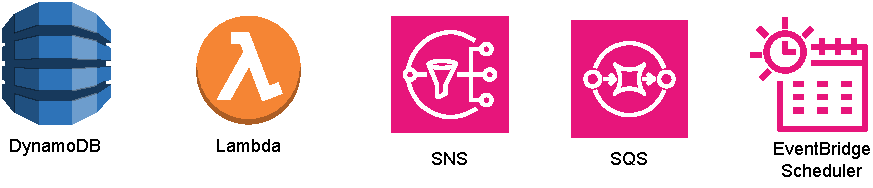
\includegraphics[width=0.95\textwidth,keepaspectratio]{../images/AWS_components.pdf}
    \caption{AWS diagram component labelling}
    \label{fig:awsComponents}
\end{figure}
\subsection{Security}
Software Security is important, especially in the context of this project that deals with sensitive health data. Generic web-accessible recommendations should apply to this project, such as encryption, xss, etc. However, deploying the application on the cloud presents new security related challenges, which a lot of companies suffer from [cite]. 
\section{LLMs}
"A large language model is the language model with massive
parameters that undergoes pretraining tasks (e.g., masked
language modeling and autoregressive prediction) to un-
derstand and process human language, by modeling the
contextualized text semantics and probabilities from large
amounts of text data " \cite{Yao2023ASO}
Unlike neural networks, the main way to improve response quality is to improve the prompt \cite{Liu2021PretrainPA}; "Prompt Engineering" is the technique for doing that, maximizing utility of LLMs in various tasks \cite{zhou2023large}. The following techniques were discovered:
\begin{itemize}
   \item Retrieval Augmented Generation (RAG): RAG is a functionality that allows LLMs to access relevant external knowledge and use it for response generation. It is usually more prioritised that the ordinary context,significantly reducing the chances of hallucinations and improving output quality \cite{gao2024retrievalaugmented}.
   \item Few Shot prompting: Also called in-context learning, providing hand-crafted examples of good replies to an input, has shown to provide better model performance; however it still struggles with complex reasoning tasks \cite{brown2020language, min2022rethinking}. When 1 pair is provided it is called 1-shot prompt, 5 - 5-shot, etc. 
   \item Chain of Thought (CoT) prompting: when utilising few shot prompting, providing intermediate reasoning steps in the example reply has shown to improve performance as well as enabling complex reasoning capabilities \cite{wei2023chainofthought}. It is also possible in a zero-shot prompt i.e prompt without examples, by providing this "magic" phrase at the end of the prompt: "Let's think step by step"; This has shown to improve performance over default prompt and rival few-shot prompts \cite{kojima2023large}.
\end{itemize}
 In 2022, OpenAI made GPT3 available to the public, a product that surpassed Google in daily webpage visits. It revolutionized AI, in a way that a lay person could use it with some decent efficiency. The vital factor is it's ability to effectively utilize context window, a collection of prior information (such as prior messages sent in a chat) that is used to influence the next output. The workflow of using GPT3 as a software developer is as follows: Explicitly attach context messages together with a prompt. The complexity of managing contexts was upon your system that uses the OpenAI API. This recently changed with Assistants API. This feature allows creating of assistants, which can have threads that correspond to continuous chat with a user. Key factor is that the complexity of maintaining context is handled by OpenAI. Also it features OpenAI's own Retrieval Assisted Generation (RAG) solution named Knowledge Retrieval. 


\section{Data analysis \& Statistical Testing}
\subsection{Bland-Altman Plot}
Bland-Altman plot is a general method for visualizing differences between measurements of two methods. The Bland-Altman (BA) graph consists of a scatter plot in which the difference between two measures (Test \#1 - Test \#2) is constructed on the vertical axis, while the mean of the two measures ([Test \#1 + Test \#2]/2) is depicted on the horizontal axis \cite{kaur2017bland}. Limits of agreement may also be drawn. They signify boundaries of difference, beyond which points would be more than x standard deviations away from the mean difference; 1.96 SD is commonly used \cite{myles2007using}.  In particular, it is used extensively in medical research, when there is a need to determine if two methods can be used interchangeably \cite{myles2007using}.
\subsection{Outlier detection - Z-score}
Z-score or also known as Standard score, is the number of standard deviations by which a data point is above or below the mean of the population. Ideally, it requires knowing population mean and standard deviation (SD), however, for practical reasons those are estimated by sample's mean SD; It is calculated by: $z=\frac{x-\hat{x}}{SD}$ \cite{zscoreBook}. It can be used for outlier detection, such as data points more than 2 SDs away are considered outliers, i.e data points with $\text{abs}(z) >= 2$ are outliers.
\subsection{Hypothesis testing}
Student's t-test is a statistical testing method to test a hypothesis of whether population means of 2 groups are different with a certain confidence. It is often the preffered choice over Z-test, as it does not require knowing population's mean and SD; instead those are estimated from the sample and corrected with degrees of freedom according to the sample size. The normal version, also called Independent t-test assumes equal variance between 2 groups, whereas Paired version does not assume equal variance. Paired version should be used when two groups depend on one another. \cite{LIVINGSTON200458}. 

Two one-sided test (TOST) also allows testing whether population means of 2 groups are different, however we can also define bounds on what is considered a worthwhile difference - these are called equivalence bounds; if the difference between 2 groups is within those defined lower and upper equivalence bounds at a certain confidence, the difference is not too interesting. Basically we can test whether the difference between groups is significantly more than some defined tolerance values, instead of just testing whether difference is more. \cite{tost}.
% On 4th March 2024, Shortly after finishing the project implementation, Anthropic announced Claude 3 Sonnet. It's benchmark scores are similar or better than gpt-4-1106-preview, it has bigger context window but costs 333\% less. This makes the reasoning behind the choice of gpt-4-1106-preview not valid at the moment of writing the report, however it was valid at the time of planning for AI functionality at the time of Dec 2023. 